As previously mentioned in this document, the System can be divided into three main part: the Core, the Website and the Mobile App + Smartwatch App. More specifically:
\begin{itemize}
    \item \textbf{Frontend components:} contains the Smartwatch App, the Mobile App and the Website.
    \item \textbf{Backend components:} contains the Core with all its components and the DBMS.
    \item \textbf{External components:} contains all the external components, such as the Payment Service, the communication with the Ambulance system and so on.
\end{itemize}

\noindent In order to implement, integrate and test the system, a \textit{Bottom-up approach} will be used. In this way, the different subsystems can be implemented independently one from each other. As the dependencies of each subsystem are developed, the various subsystems can be progressively integrated and tested.\\
For what concerning the Mobile App and the Website, these can be implemented assuming that the Core is fully working and running, as they interact only using REST api (i.e. a stub server with mockup responses can be used as these are fully formalized in this document). Only when the Core is fully developed and tested an integration test can be made.

The components to be implemented, integrated and tested are, in order:
\begin{enumerate}
    \item DBMS \& Storage Manager;
    \item Authentication Manager, along with Mail interface;
    \item Individual Manager, along with Push Notification interface;
    \item Subscription Manager, along with the Payment interface;
    \item Query Manager, with integration with Push Notification;
    \item Emergency Manager, along with Emergency interface;
    \item Run Manager, with integration with Individual manager.
\end{enumerate}

\label{CD}

As the Core integration and testing is finished, the integration between the Website and the Core and the Smartphone App and the Core can be made in this order:
\begin{enumerate}
    \item Website, Mobile App with Authentication manager;
    \item Mobile App with Individual manager;
    \item Website with Subscription manager;
    \item Website with Query manager;
    \item Mobile App with Run manager.
\end{enumerate}













\subsection{Sequence of component integration}
The diagrams below describe the sequence of the component implementation, integration and testing of the system.

\paragraph{Integration of the backend}
Firstly all the components will be implemented and tested with unit tests.
Database and Storage manager are the firsts to be implemented and tested because they offer methods to access data.
Then the integration process will proceed in the following order:





\begin{figure}[H]
	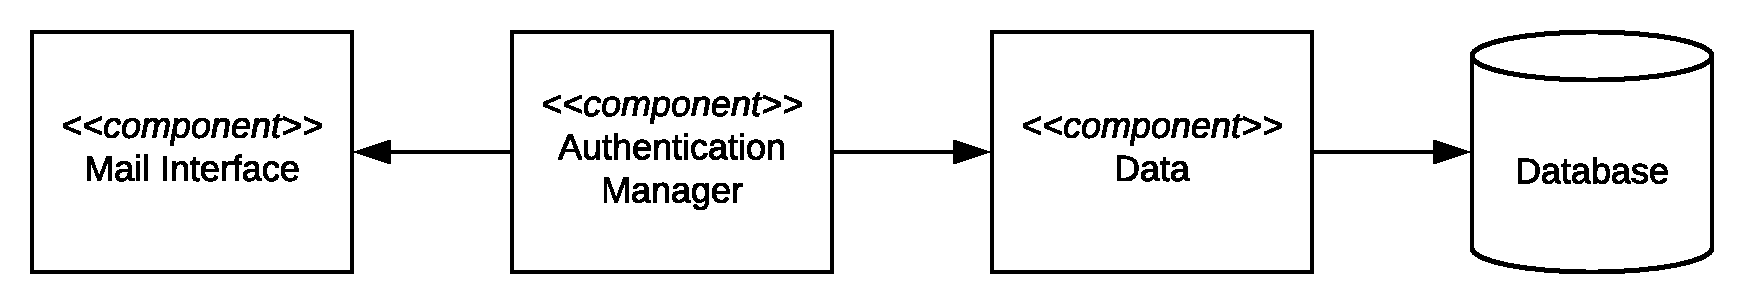
\includegraphics[width=\textwidth,height=\textheight,keepaspectratio]{assets/integration/AuthDataMail.pdf}
	\caption{Auth Manager integration}
	\label{fig:AuthDataMail}
\end{figure}



\begin{figure}[H]
	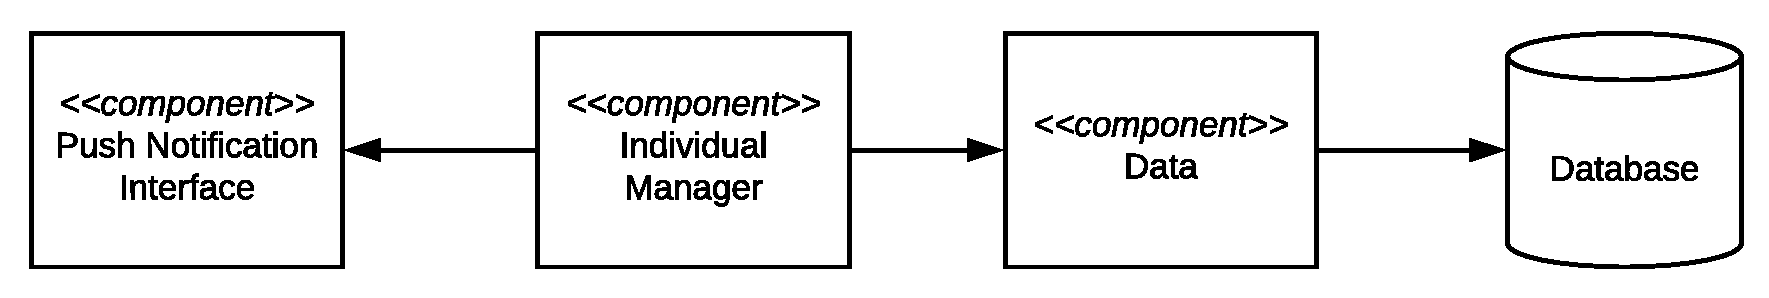
\includegraphics[width=\textwidth,height=\textheight,keepaspectratio]{assets/integration/IndividualPush.pdf}
	\caption{Individual Manager integration}
	\label{fig:IndividualPush}
\end{figure}

\begin{figure}[H]
	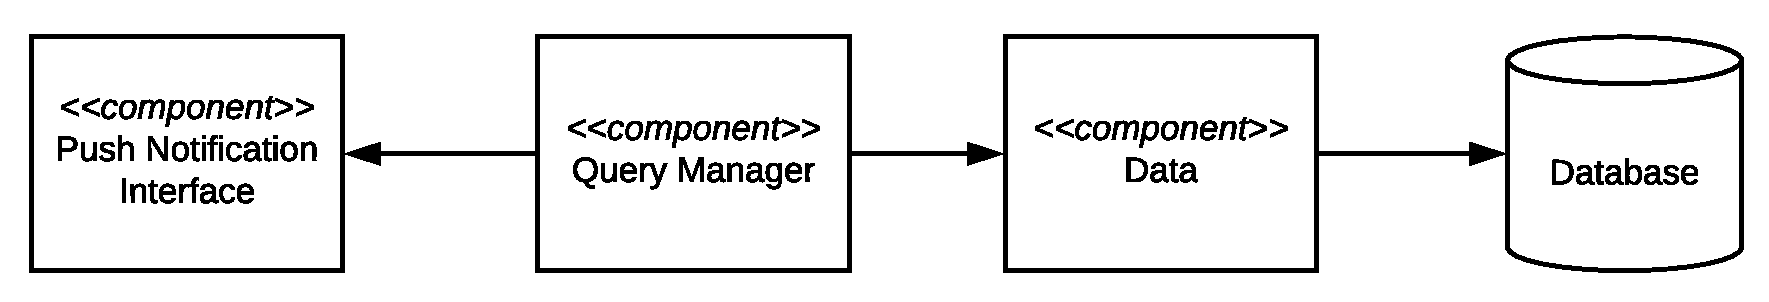
\includegraphics[width=\textwidth,height=\textheight,keepaspectratio]{assets/integration/QueryPush.pdf}
	\caption{Query Manager integration}
	\label{fig:QueryPush}
\end{figure}



\begin{figure}[H]
	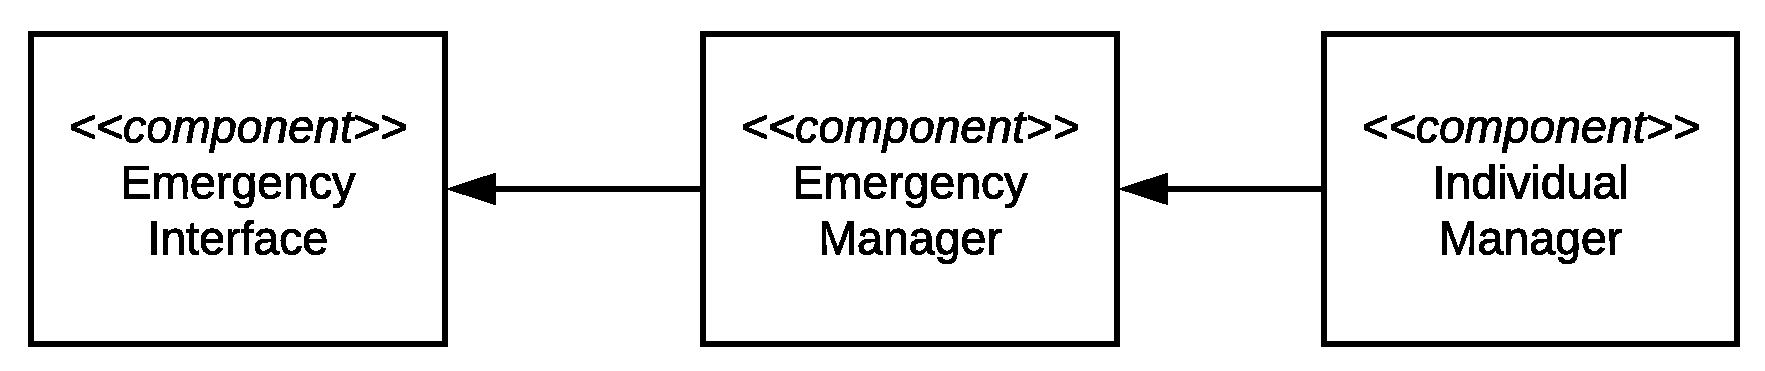
\includegraphics[width=\textwidth,height=\textheight,keepaspectratio]{assets/integration/EmergencyIndividual.pdf}
	\caption{Emergencency Manager integration}
	\label{fig:EmergencyIndividual}
\end{figure}


\begin{figure}[H]
	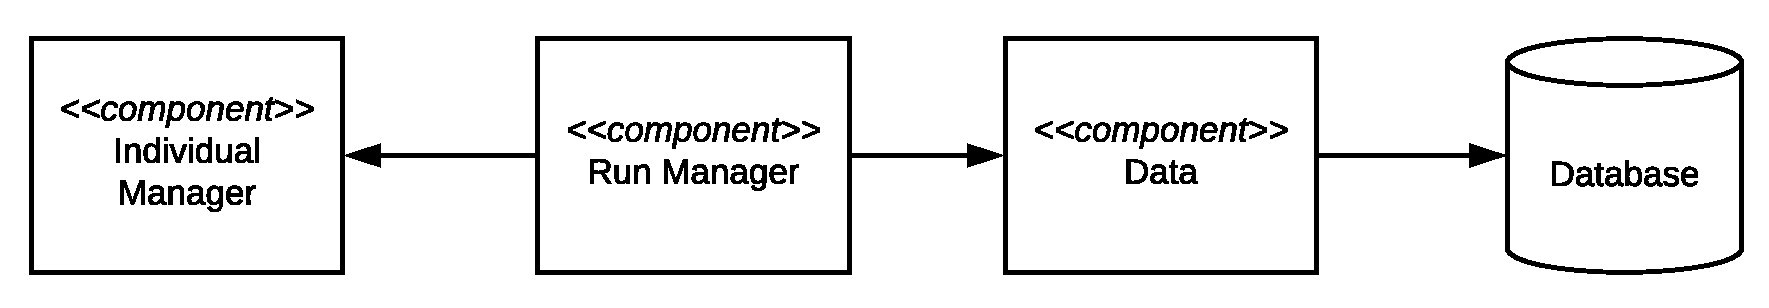
\includegraphics[width=\textwidth,height=\textheight,keepaspectratio]{assets/integration/IndividualRun.pdf}
	\caption{Run Manager Integration}
	\label{fig:IndividualRun}
\end{figure}

\noindent In order to have the main functionality tested, we expect to integrate the external interfaces at the same time with the integration with other internal components.




\paragraph{Integration of the frontend with backend}
Once all the components of the backend are implemented and tested among each others, the frontend will be integrated and tested within the backend. \\
The subsystems to be integrated are 2:
\begin{itemize}
    \item The Website Client, that interacts with the Authentication Manager, Query Manager, Subscription Manager;
    \item The Mobile app Client, that interacts with the Run Manager, Authentication Manager, and Individual Manager
\end{itemize}

\begin{figure}[H]
	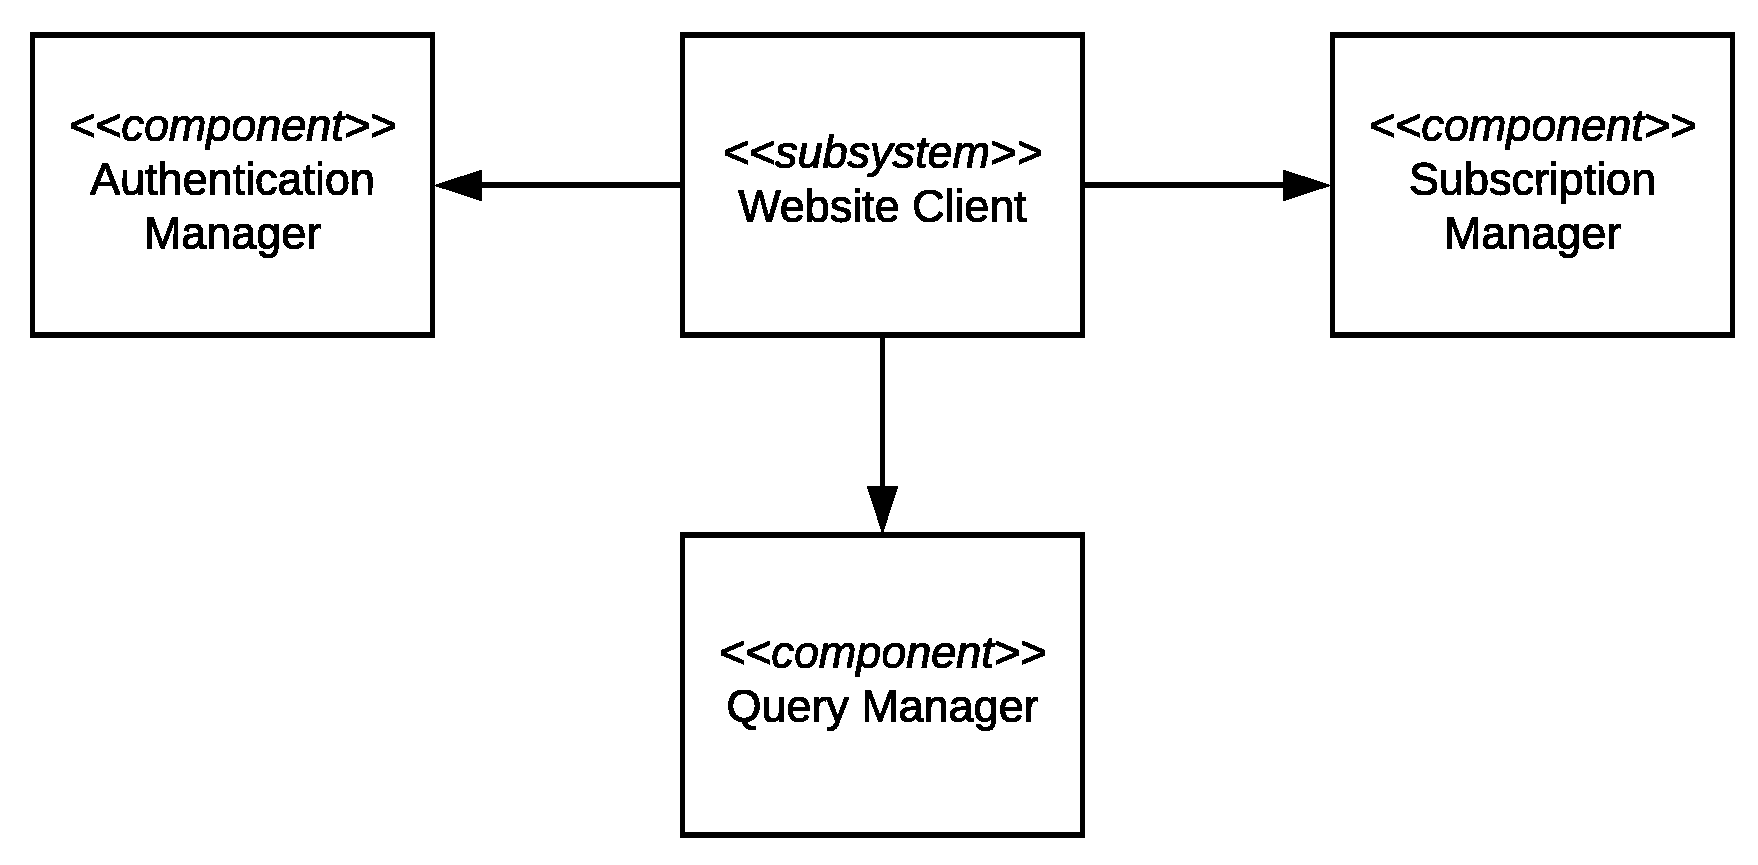
\includegraphics[width=\textwidth,height=\textheight,keepaspectratio]{assets/integration/IntegrationWebsite.pdf}
	\caption{Website integration}
	\label{fig:IntegrationWebsite}
\end{figure}

\begin{figure}[H]
	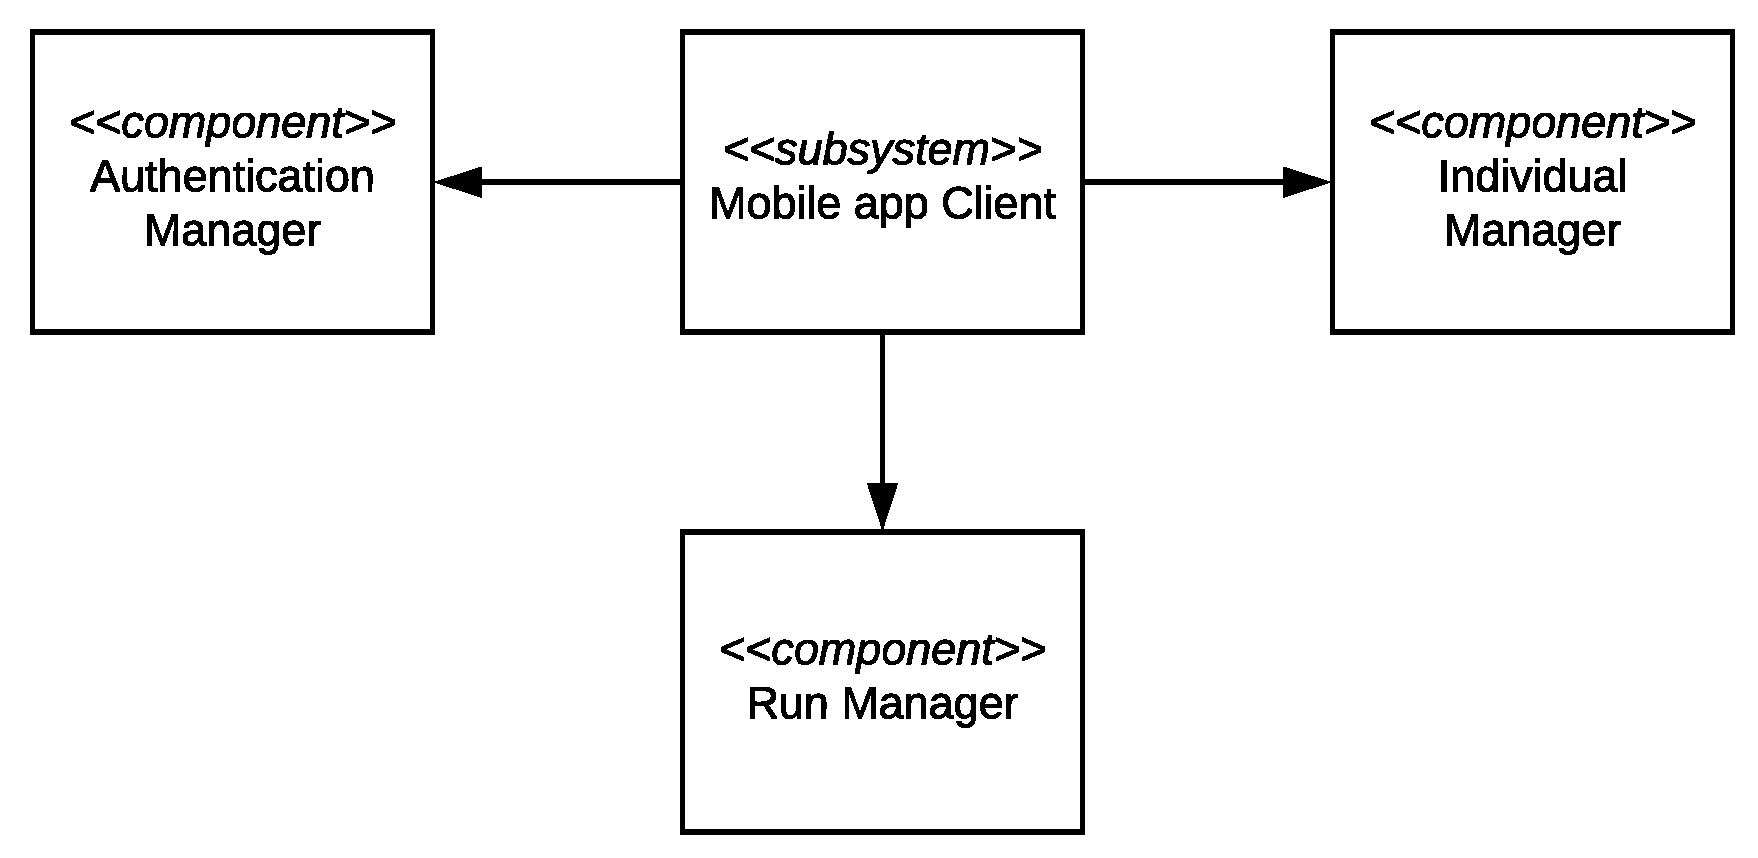
\includegraphics[width=\textwidth,height=\textheight,keepaspectratio]{assets/integration/IntegrationMobileApp.pdf}
	\caption{Mobile App integration}
	\label{fig:IntegrationMobileApp}
\end{figure}


\paragraph{Integration of all subsystems}
Once the front-end has been integrated with the Back-end, the system will be fully tested, with the respect of all the components shown in the \nameref{fig:CD}.

